% ---------------------------------------------------------------------------
% [FIGURE] ecf_teaser   spec: results/xtragpt/RELAYOUT_PLAN_and_FIGURE_SUITE.md Sec. 3.1 (F1)
% after the figure exists, replace this block with the rendered figure file figures/ecf_teaser_redraw.png
% ---------------------------------------------------------------------------
\begin{figure*}[t]
\centering
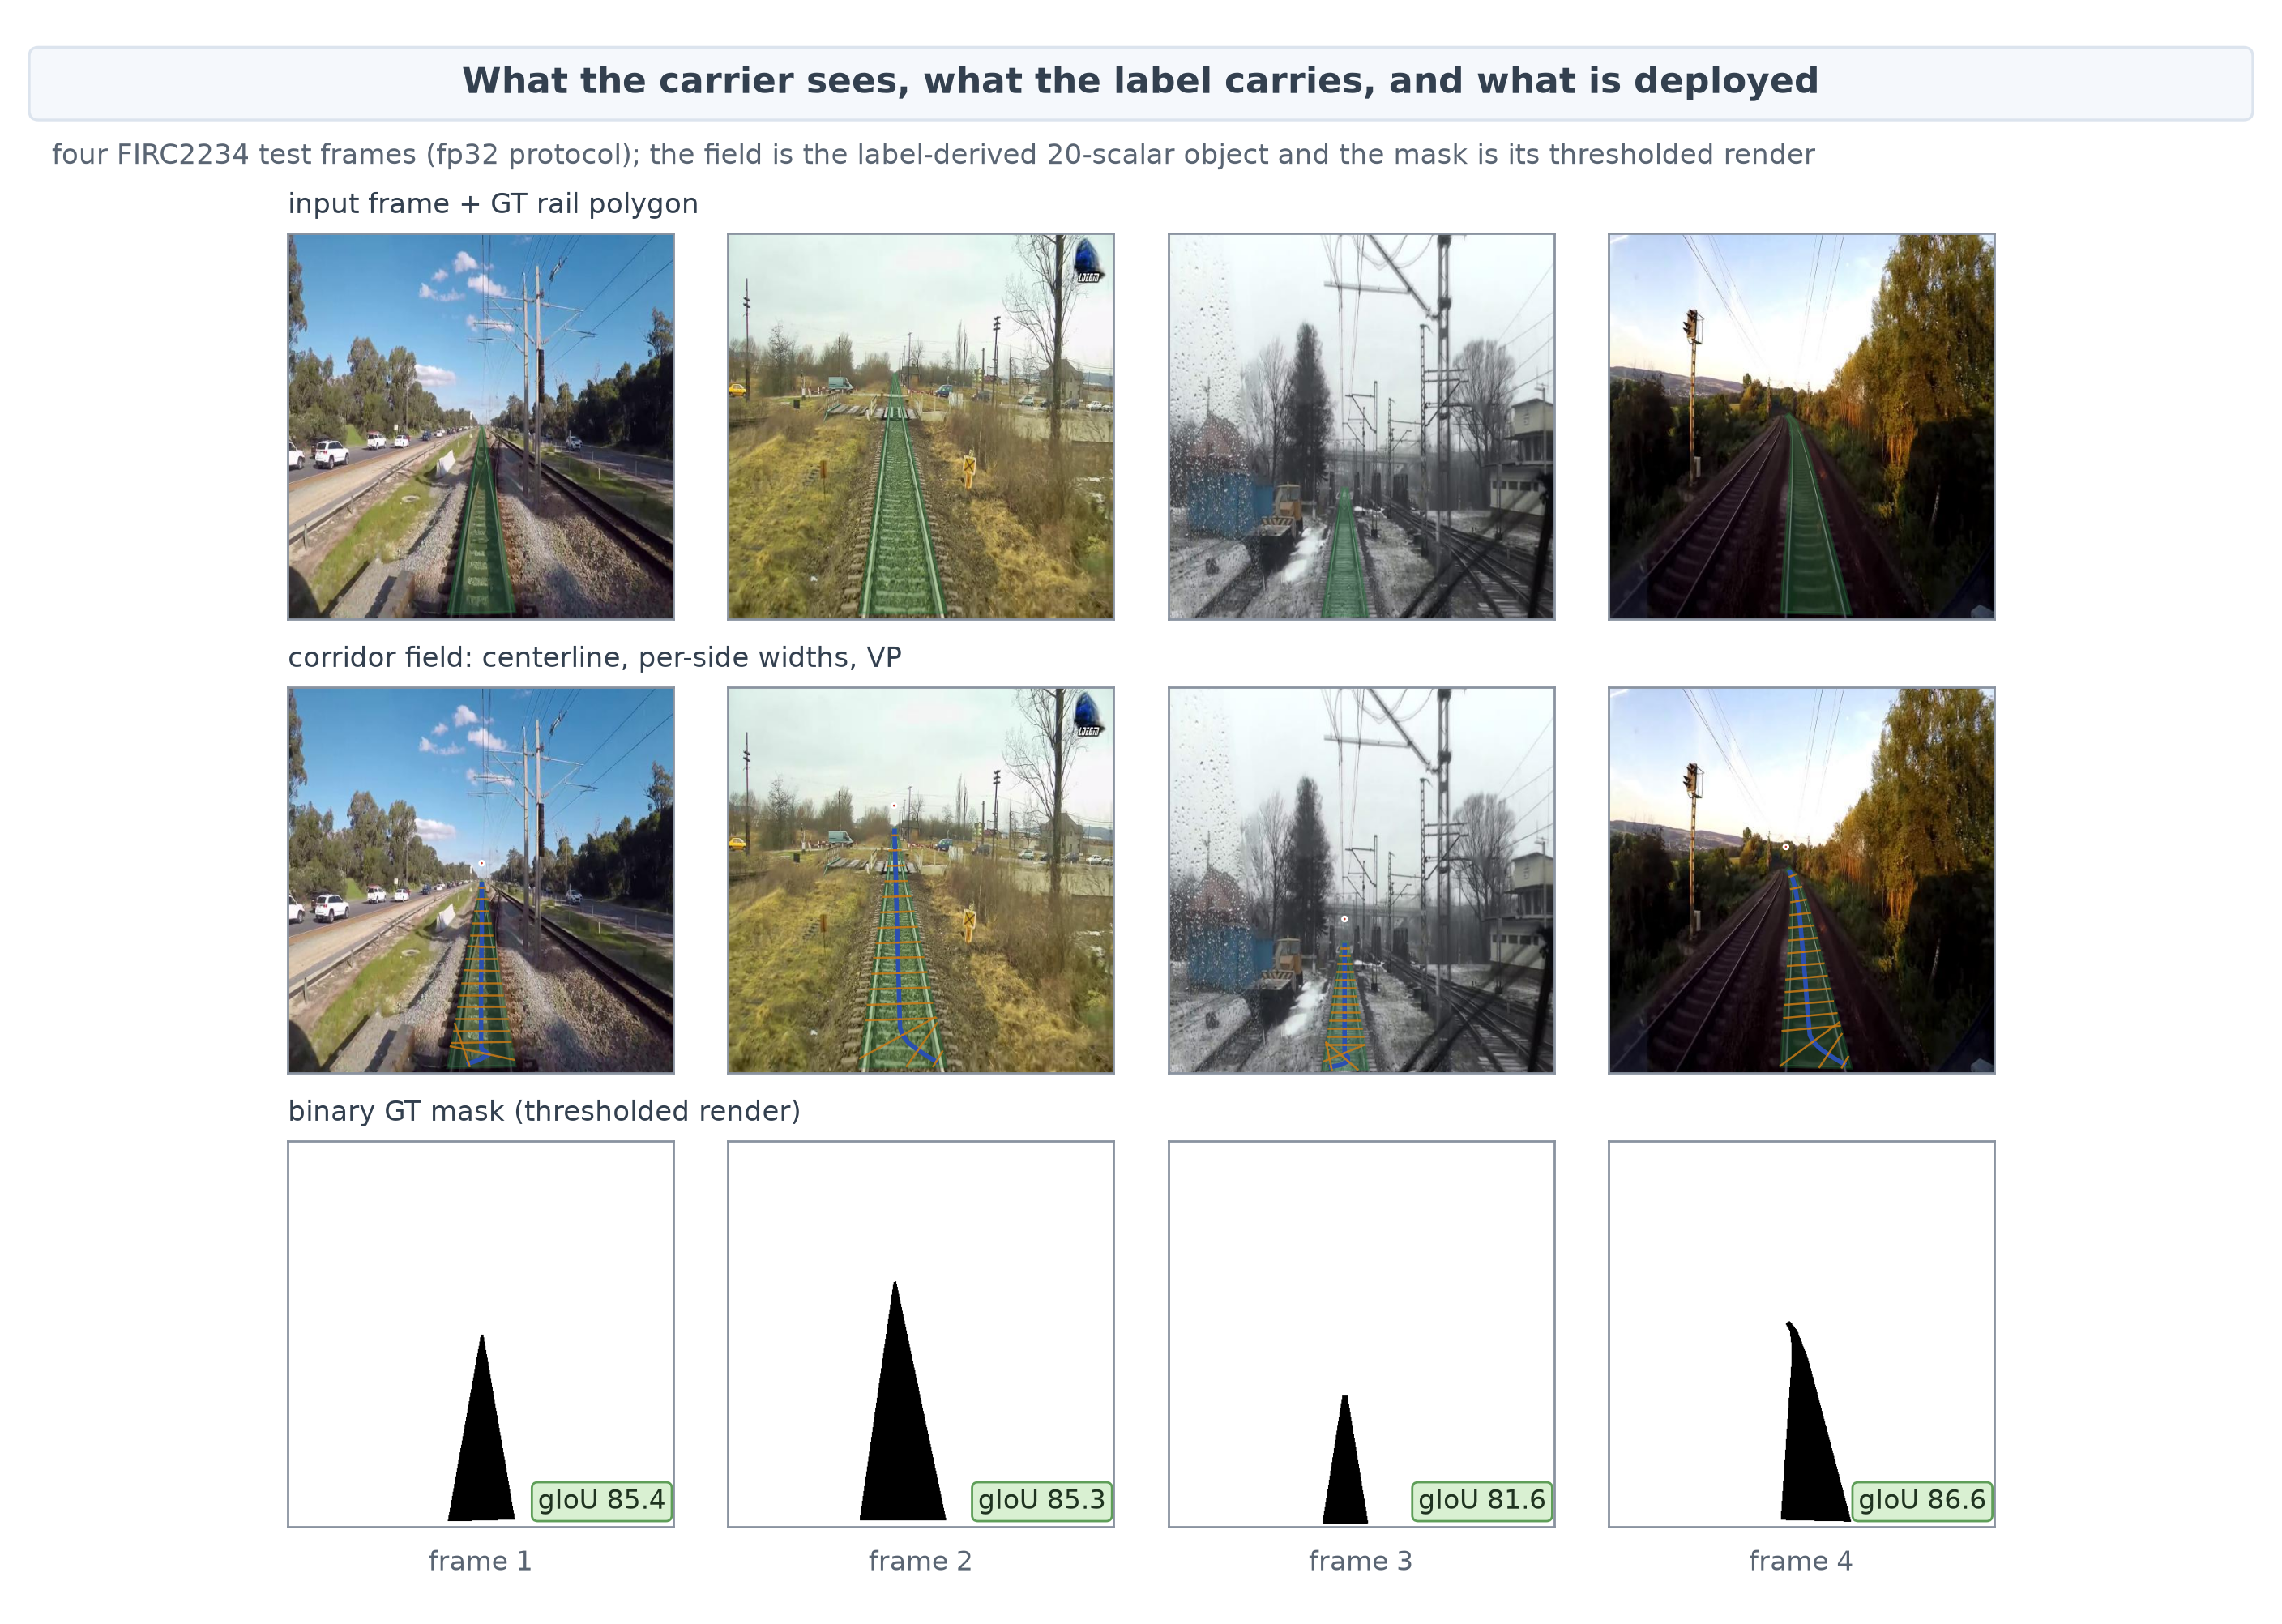
\includegraphics[width=\textwidth]{figures/ecf_teaser_redraw.png}
\caption{Capability of the corridor-field carrier on four ego-view rail settings. Each column shows the input frame, the predicted field overlaid as a centerline with a vanishing point, and the deployed binary mask; no mask on this path is decoded by SAM2.}
\label{fig:ph_ecf_teaser}
\end{figure*}

\begin{figure*}[t]
\centering
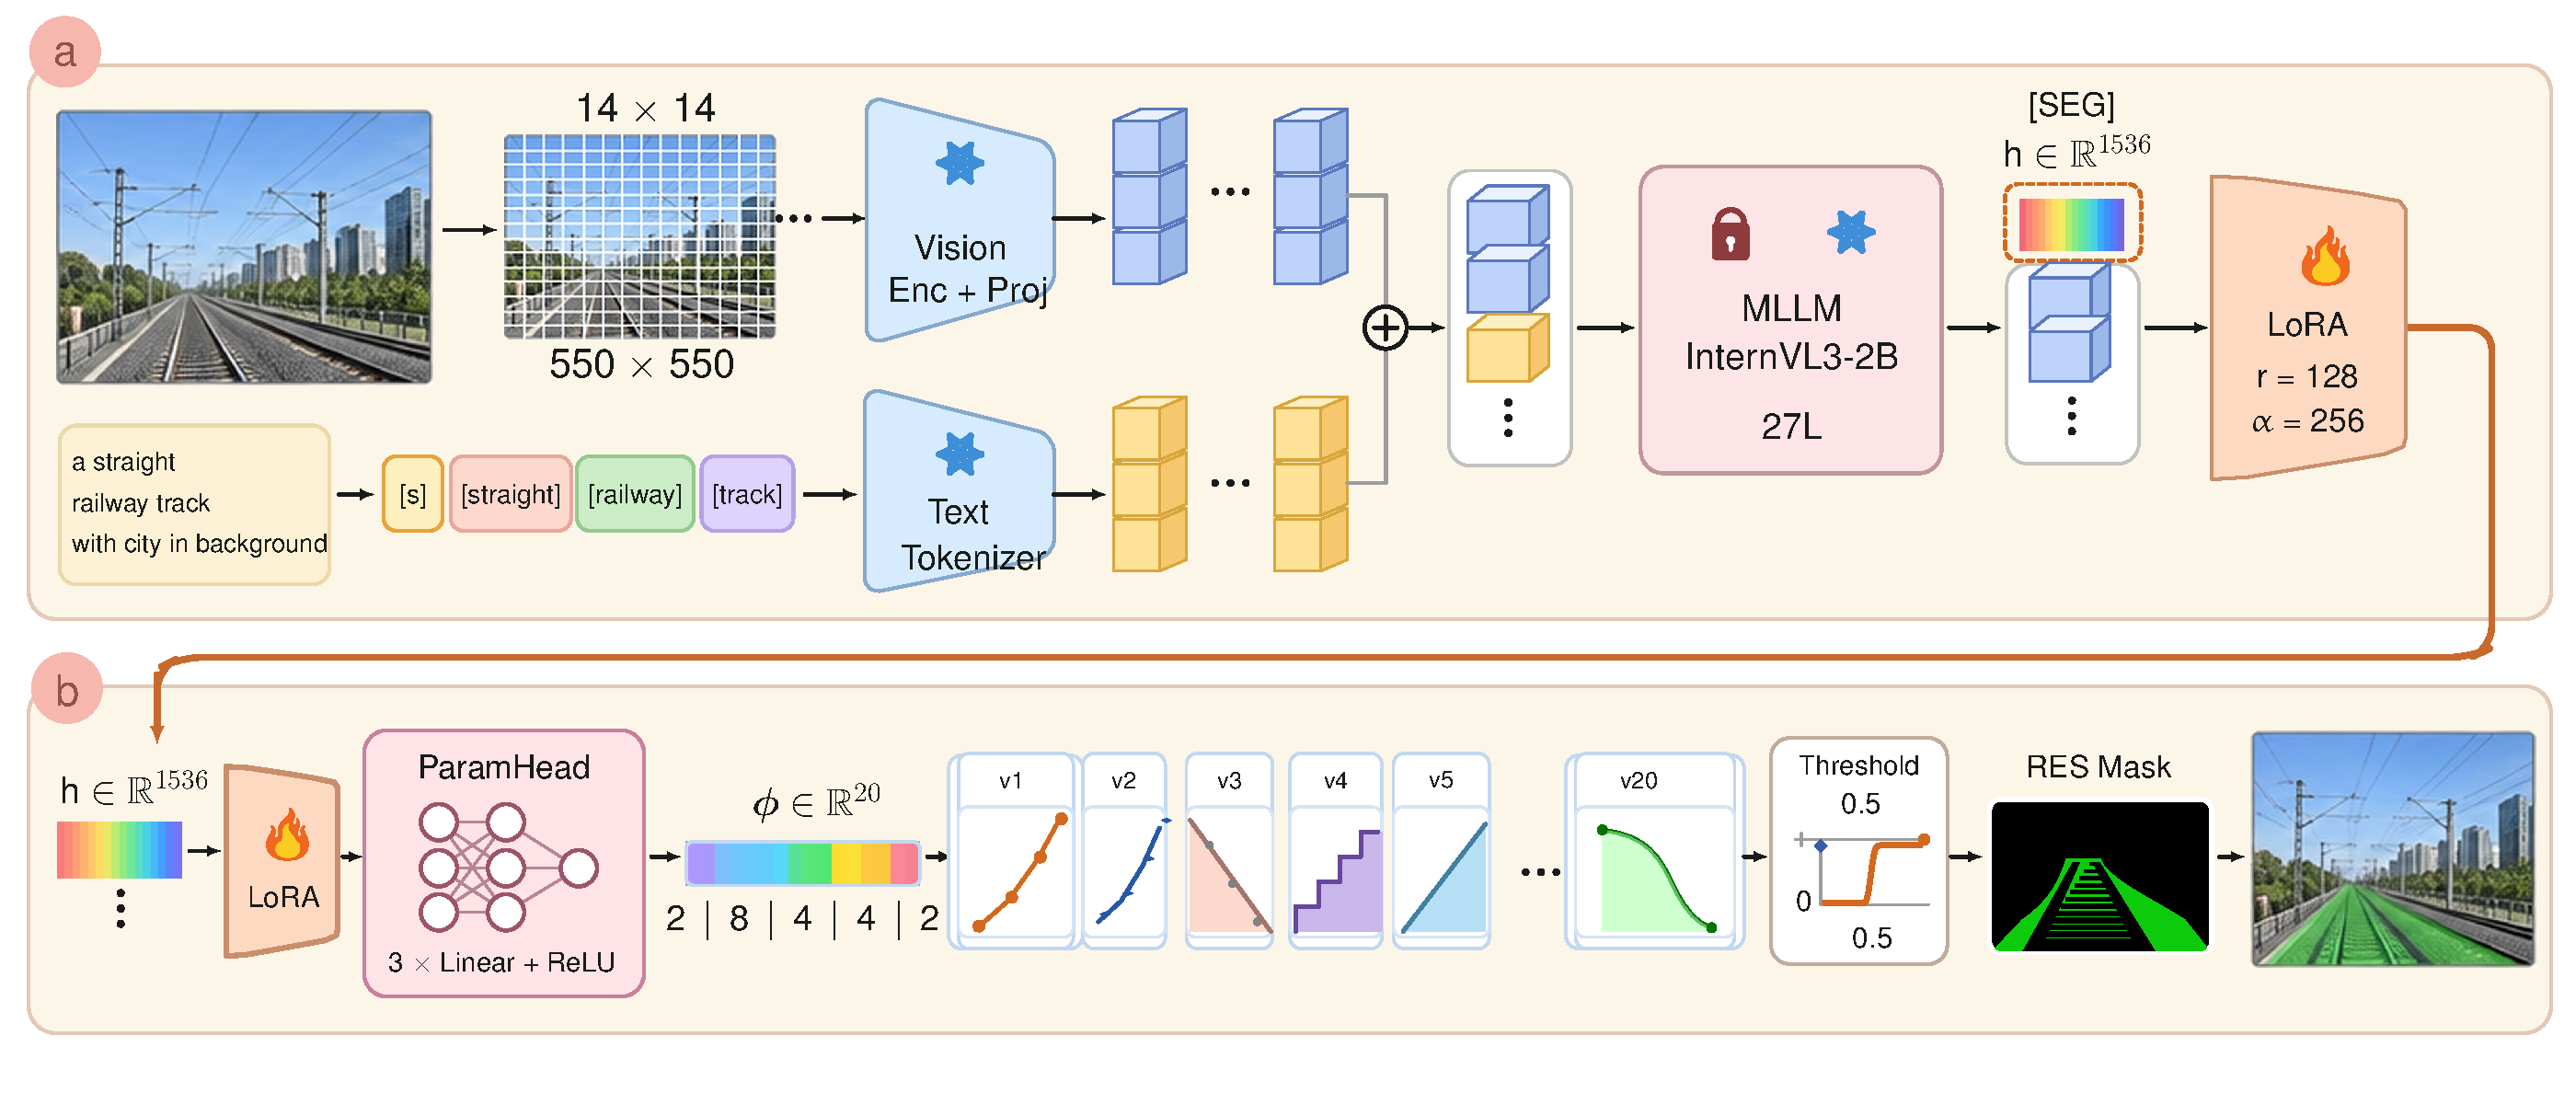
\includegraphics[width=\textwidth]{figures/ecf_forward_vec.pdf}%
\caption{Forward detail of the corridor head.
(a)~the referring frame through the frozen Sa2VA trunk (vision encoder and text tokenizer into the InternVL3-2B MLLM, whose first \Seg{} hidden state $h \in \mathbb{R}^{1536}$ is read by the LoRA-adapted head);
(b)~ParamHead (three linear layers with ReLU) maps $h$ to the corridor scalars $\phih$, which the differentiable rasterizer consumes slot by slot (vanishing point, $c_{1:K}$ centerline, left/right width samples, topology logits) to produce the soft mask and the thresholded RES mask.
Intended as a pictorial complement to Eq.~\eqref{eq:phi}: the slots are drawn as individual control curves to make the low-dimensional parameterization explicit.}
\label{fig:ecf_forward}
\end{figure*}

Figure~\ref{fig:ph_ecf_teaser} shows what the carrier produces across four ego-view rail settings, and Table~\ref{tab:quant} places it against the off-the-shelf reference set with the gIoU ratio to our row.


\begin{table}[t]
\centering
\small
\setlength{\tabcolsep}{4pt}
\caption{Accuracy and the gIoU ratio to our row (FIRC2234 test, fp32, $n{=}208$). Rows 2--4 are the off-the-shelf reference set of Table~\ref{tab:main}, measured by us on the same protocol; the ratio column gives our gIoU divided by the row's. A1 decodes the same trained $h$ with SAM2 (Table~\ref{tab:ablate}).}
\label{tab:quant}
\begin{tabularx}{\columnwidth}{@{}Ycc@{}}
\toprule
Method & \gIou & Ratio vs ours \\
\midrule
\textbf{Ours: ECF-native $\phih{\to}\cR$} & \textbf{80.67} & \textbf{$1.0\times$} \\
GroundingDINO+SAM2~\citep{liu2024groundingdino} & 28.18 & $2.9\times$ \\
Qwen2.5-VL-7B+SAM2~\citep{bai2025qwen2vl} & 25.60 & $3.2\times$ \\
Sa2VA pretrained~\citep{zhang2025sa2va} (no fine-tuning) & 14.32 & $5.6\times$ \\
A1: same $h$, SAM2 decode & 2.43 & -- \\
\bottomrule
\end{tabularx}
\end{table}

\section{Related Work}
\label{sec:related}

\paragraph{Referring expression segmentation and the \Seg{} interface.}
RES requires segmenting the object described by a natural-language expression, classically benchmarked on RefCOCO, RefCOCO+, and RefCOCOg \citep{yu2016refcoco,mao2016refcocog}.
The field has moved from proposal-matching pipelines to MLLM-based systems: LISA \citep{lai2024lisa} adds reasoning capability on top of SAM-style decoding, GLaMM \citep{rasheed2024glamm} unifies grounding with pixel-level generation, and Sa2VA \citep{zhang2025sa2va} marries LLaVA-class language models with SAM2 \citep{ravi2024sam2}, decoding \Seg{} tokens into masks through a frozen image encoder.
A parallel trend in generalist segmentation is to attach many task heads to a single foundation backbone: GLEE \citep{wu2024glee} unifies object-level tasks across images and videos, and SAM-Track \citep{cheng2023samtrack} chains SAM with a tracker for interactive video segmentation.
These systems keep a dense mask decoder as the carrier and vary what is fed into it; they supervise an arbitrary-shaped target as a dense mask.
The RES literature extends beyond dense decoding: PolyFormer predicts polygon vertices rather than pixels \citep{liu2023polyformer}, GRES extends the task to multi-target and no-target expressions with the region-based baseline ReLA \citep{liu2023gres}, and referring video object segmentation carries the caption-to-object interface to video \citep{miao2024htr}. PolyFormer is the closest parametric output, but its polygons come from a task-specific decoder, not from a referring token inside an MLLM.
We vary the carrier itself, for a target class whose shape is a \emph{perspective corridor}: in a calibrated ego view the referred rail is a vanishing-point-anchored centerline with a bilateral width field, and it is this low-dimensional structure, not a free silhouette, that the token is asked to emit.

DeSa2VA \citep{dang2025desa2va} is the closest architectural diagnosis of this interface, arguing that Sa2VA's shared \Seg{} token (i)~carries insufficient semantics, (ii)~is consumed by a SAM2 decoder that was never trained on text, and (iii)~provides only a sparse high-level hint rather than a fine-grained visual prompt.
The proposed remedy is linear decoupling of MLLM hidden states, a text-derived mask pre-training stage that turns labels into rasterized text masks for SAM2, and a one-step mask-reprompt loop.
On RefCOCO/+/g, its authors report that DeSa2VA-4B improves Sa2VA-4B by 3.7/6.1/5.1 points (82.6 / 77.8 / 79.2 versus 78.9 / 71.7 / 74.1), and their ablation additionally shows that \emph{text-derived mask pre-training of SAM2 without decoupling hurts} Sa2VA (RefCOCO 78.9$\to$73.4).
We keep the original Sa2VA token and do not add a decoupling module, and we make no claim that decoupling is unnecessary in general: our scope is targets whose shape is a perspective corridor, where the carrier can be parameterized directly.
What we change is what the token is allowed to mean---not a SAM2 prompt, but the parameters of a corridor field.
The two treatments act at different points of the same interface: DeSa2VA enriches the encoder-side prompt that SAM2 receives, and we replace SAM2 as the mask carrier; we read them as alternatives for different target classes rather than as a refutation.

\paragraph{Parametric lanes and differentiable rasterization.}
Ego-view lane and corridor estimation has long used low-dimensional models rather than free masks: polynomial or B\'ezier centerlines \citep{tabelini2021polylanenet,feng2022bezierlanenet}, perspective-aware transformers \citep{chen2022persformer}, cross-layer refinement \citep{zheng2022clrnet}, and conditional kernels that explicitly cover lane forks \citep{liu2021condlanenet}.
Those systems are detectors or segmenters with a geometric head; they are not MLLM referring models and they do not have to bind an ordinal caption to one of several parallel rails.
We import the geometric \emph{carrier} (a centerline plus bilateral width, carried alongside a vanishing-point slot) into a Sa2VA \Seg{} token.
The map from parameters to pixels is a differentiable rasterizer in the spirit of soft rendering \citep{kato2018renderer,liu2019softras}: occupancy is a sigmoid of signed distance to the polyline, so mask losses back-propagate into $\phih$.

\paragraph{Fine-grained special tokens.}
Momentor++ \citep{li2026momentorpp} shows that Video-LLM localization tokens only become useful after an intermediate grounded-processing stage; without it, discrete special tokens collapse into unrelated embeddings.
We do not implement temporal tokens; we borrow the observation that a special localization token is not by itself a complete spatial representation---for \Seg{}, DeSa2VA's sparse-prompt claim---and put the missing spatial detail into $\phih$ rather than into a second SAM2 stream.

\paragraph{Railway scene segmentation.}
Railway perception has its own segmentation literature, and it is the nearest neighbor of the task studied here.
RailSAM \citep{zhang2025railsam} keeps a frozen SAM encoder and injects domain geometry through multi-scale visual adapters in the mask decoder; its authors report that this parameter-efficient recipe significantly outperforms existing task-specific methods on RailSem19.
SMDE-YOLO \citep{lin2026smdeyolo} is the lightweight one-stage counterpart: Scharr-based edge enhancement, a dynamic multi-branch feature pyramid, and a decoupled segmentation head; its authors report $2.59$\,M parameters and $58.7$ FPS at $640{\times}640$ on a rail instance-segmentation benchmark.
Both solve \emph{class-level} rail segmentation, where every rail pixel is a valid ``rail'', whereas we solve expression-level target \emph{selection}: given an ordinal caption, exactly one rail is correct, and a class-level mask is a failure.
The two problems are orthogonal.
RailSAM is also a direct PEFT precedent for this paper: it shows that adapters can inject domain geometry into a generalist decoder, while ECF shows that the \Seg{} token of a referring model can emit that geometry directly instead.

\paragraph{Rail and ego-view referring scenes.}
Ego-view rail perception is a distinct regime: targets are corridor-shaped, captions are near-duplicates, and perspective creates severe pixel imbalance.
RailSem19 \citep{zendel2019railsem19} provides semantic rail-scene labels and reports rail mIoU in the 55--75 range for classical segmentation models, while detection+SAM2 pipelines built on open-vocabulary detectors \citep{liu2024groundingdino,bai2025qwen2vl} struggle with ordinal referring expressions (gIoU ${\approx}$25--28, Section~\ref{sec:exp}).
Our benchmark, FIRC2234, is a single-rail referring-segmentation corridor set with 1664/208/208 original-image splits (Figure~\ref{fig:dataset}(a)); training uses the original frames and their horizontal flips (Section~\ref{sec:data}), and two additional fill-band sets (RailSem19-EgoPair and RailBench 1L1R) are eval-only and are never mixed into the FIRC main table.

